\chapter{Cycle 2: Prototyping and Development}

\begin{chapterintro}
In this section, we discuss the findings of our second cycle where the researcher developed prototypes of a system to assist job seekers in finding employment. 
\end{chapterintro}


We began by working with participants to refine a PowerPoint-based prototype developed using Microsoft PowerPoint. Based on the overall feedback, the researcher was enacted by the participants to build a working prototype, which was developed as a web application, with an emulated wizard-of-oz backend. Section 6.1.1 discusses the PowerPoint prototype, and Section 6.2 discusses the developed prototype. Section 6.3 contains the discussions based on our findings from both prototype interactions and Section 6.4 presents a conclusion of the main points in this chapter.

%================================================
\section{High-Fidelity Prototype}

\subsection{Methods}

\begin{table}[H]
\centering
\caption{PowerPoint Prototype Walkthrough Participants}
\renewcommand{\arraystretch}{1.2}
\begin{tabularx}{\textwidth}{|X|p{2.5cm}|p{2.5cm}|p{2.2cm}|p{1.8cm}|}
\hline
\rowcolor{gray!30}
Category & Current Students & Former Students & Trainers & Total \\
\hline
Afrika Tikkun & 5 & 1 & 2 & 8 \\
\hline
The Zanokhanyo Network & 1 & 4 & 1 & 6 \\
\hline
\rowcolor{gray!15}
Total & 6 & 5 & 3 & 14 \\
\hline
\end{tabularx}
\end{table}

\FloatBarrier

For the PowerPoint prototypes, the researcher worked with 14 participants in total, eight from Afrika Tikkun and six from The Zanokhanyo Network. The participants signed consent forms and one student participant gave the researcher permission to capture a picture with her. Participants’ inputs were recorded and later transcribed.

We presented high-fidelity PowerPoint prototypes to the participants. High-fidelity prototypes were useful as they presented a clear visualization to the participants of what is possible with technology, more than would be possible with sketched paper prototypes. We performed one-on-one walkthrough sessions where we (1) presented the artefact, which was made as part of the `make` stage and (2) received feedback from the participants which was the `tell` stage.

In the `tell` phase, we gave each of our participants a chance to tell the suggestions they had on the prototype. After each participant made his/her contributions, we went on to `make` the changes. Therefore, each subsequent participant was presented with a slightly different version, based on the added changes from the previous participant.

We also presented the prototypes to trainers who gave their input to supplement what we gathered from the students (job seekers). The design suggestions from our participants enacted the creation of a testable version of the prototype — the working prototype.

In this cycle, our participants were not given any physical compensation for their time.

%================================================
\subsection{Artefact Design}

During the evaluation of the PowerPoint artefact, we were enacted to create a working prototype of the application which embodied a possible future for the job seekers, to ease how they access to job opportunities. Thus, we designed the working artefact. Figure~\ref{fig:reg1} to Figure~\ref{fig:reg3} shows the 3 pages of the user forms for job seekers to register their details on the application. The first form (Figure~\ref{fig:reg1}) prototypes taking the user’s personal details and contact information, then the second form (Figure~\ref{fig:reg2}) was designed to capture the users’ skills and qualification and finally screen 3 would capture the employment history and other identification information of the registering user. We requested the registration information in 3 parts for simplicity and to allow a maximum of 7 main aspects of memorability. Once a user has filled in the 3 screens of information, a CV and a motivational cover letter are generated automatically for the user.

\begin{figure}[h]
\centering
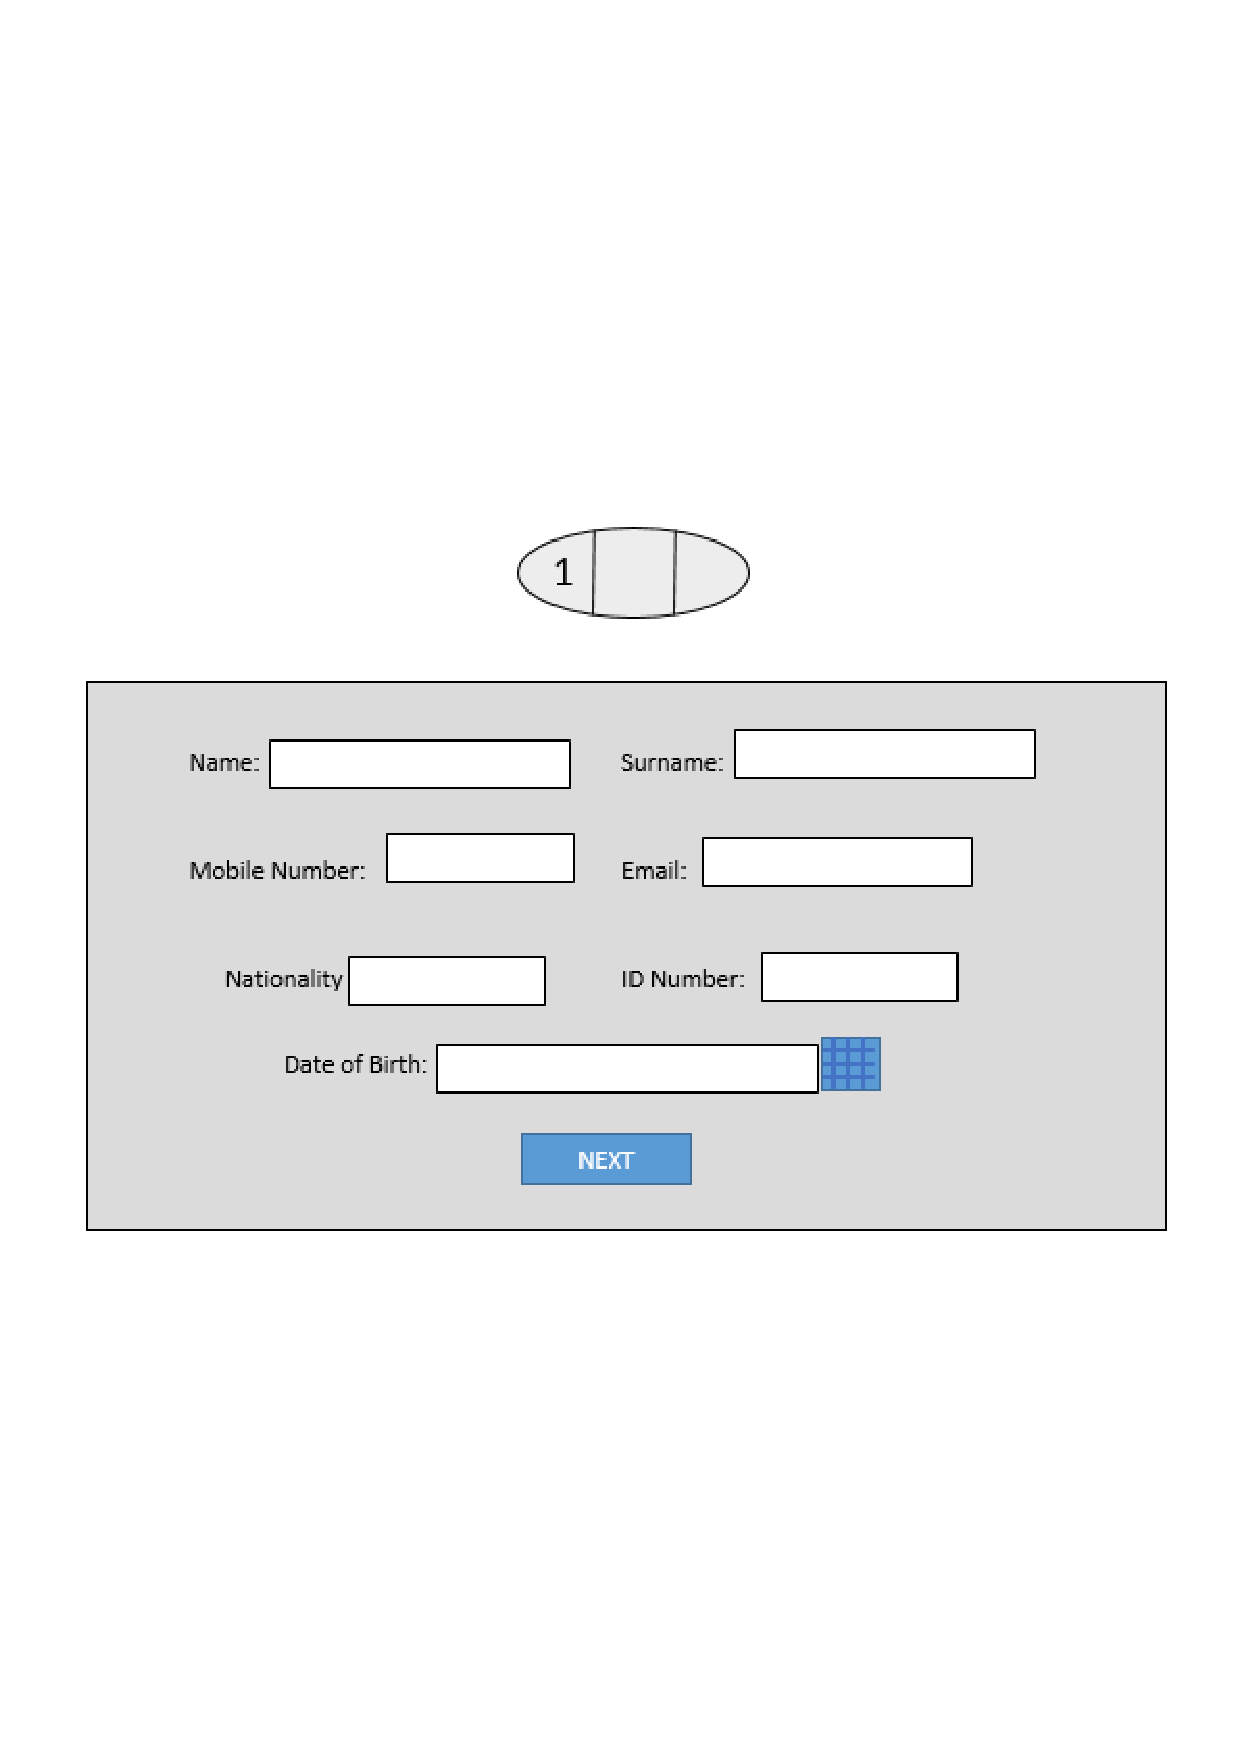
\includegraphics[width=0.7\linewidth]{dissertation/figures/Figure 3: Page 1 of 3 Registration Form Prototype.pdf}
\caption{Page 1 of 3 Registration Form Prototype}
\label{fig:reg1}
\end{figure}

\begin{figure}[h]
\centering
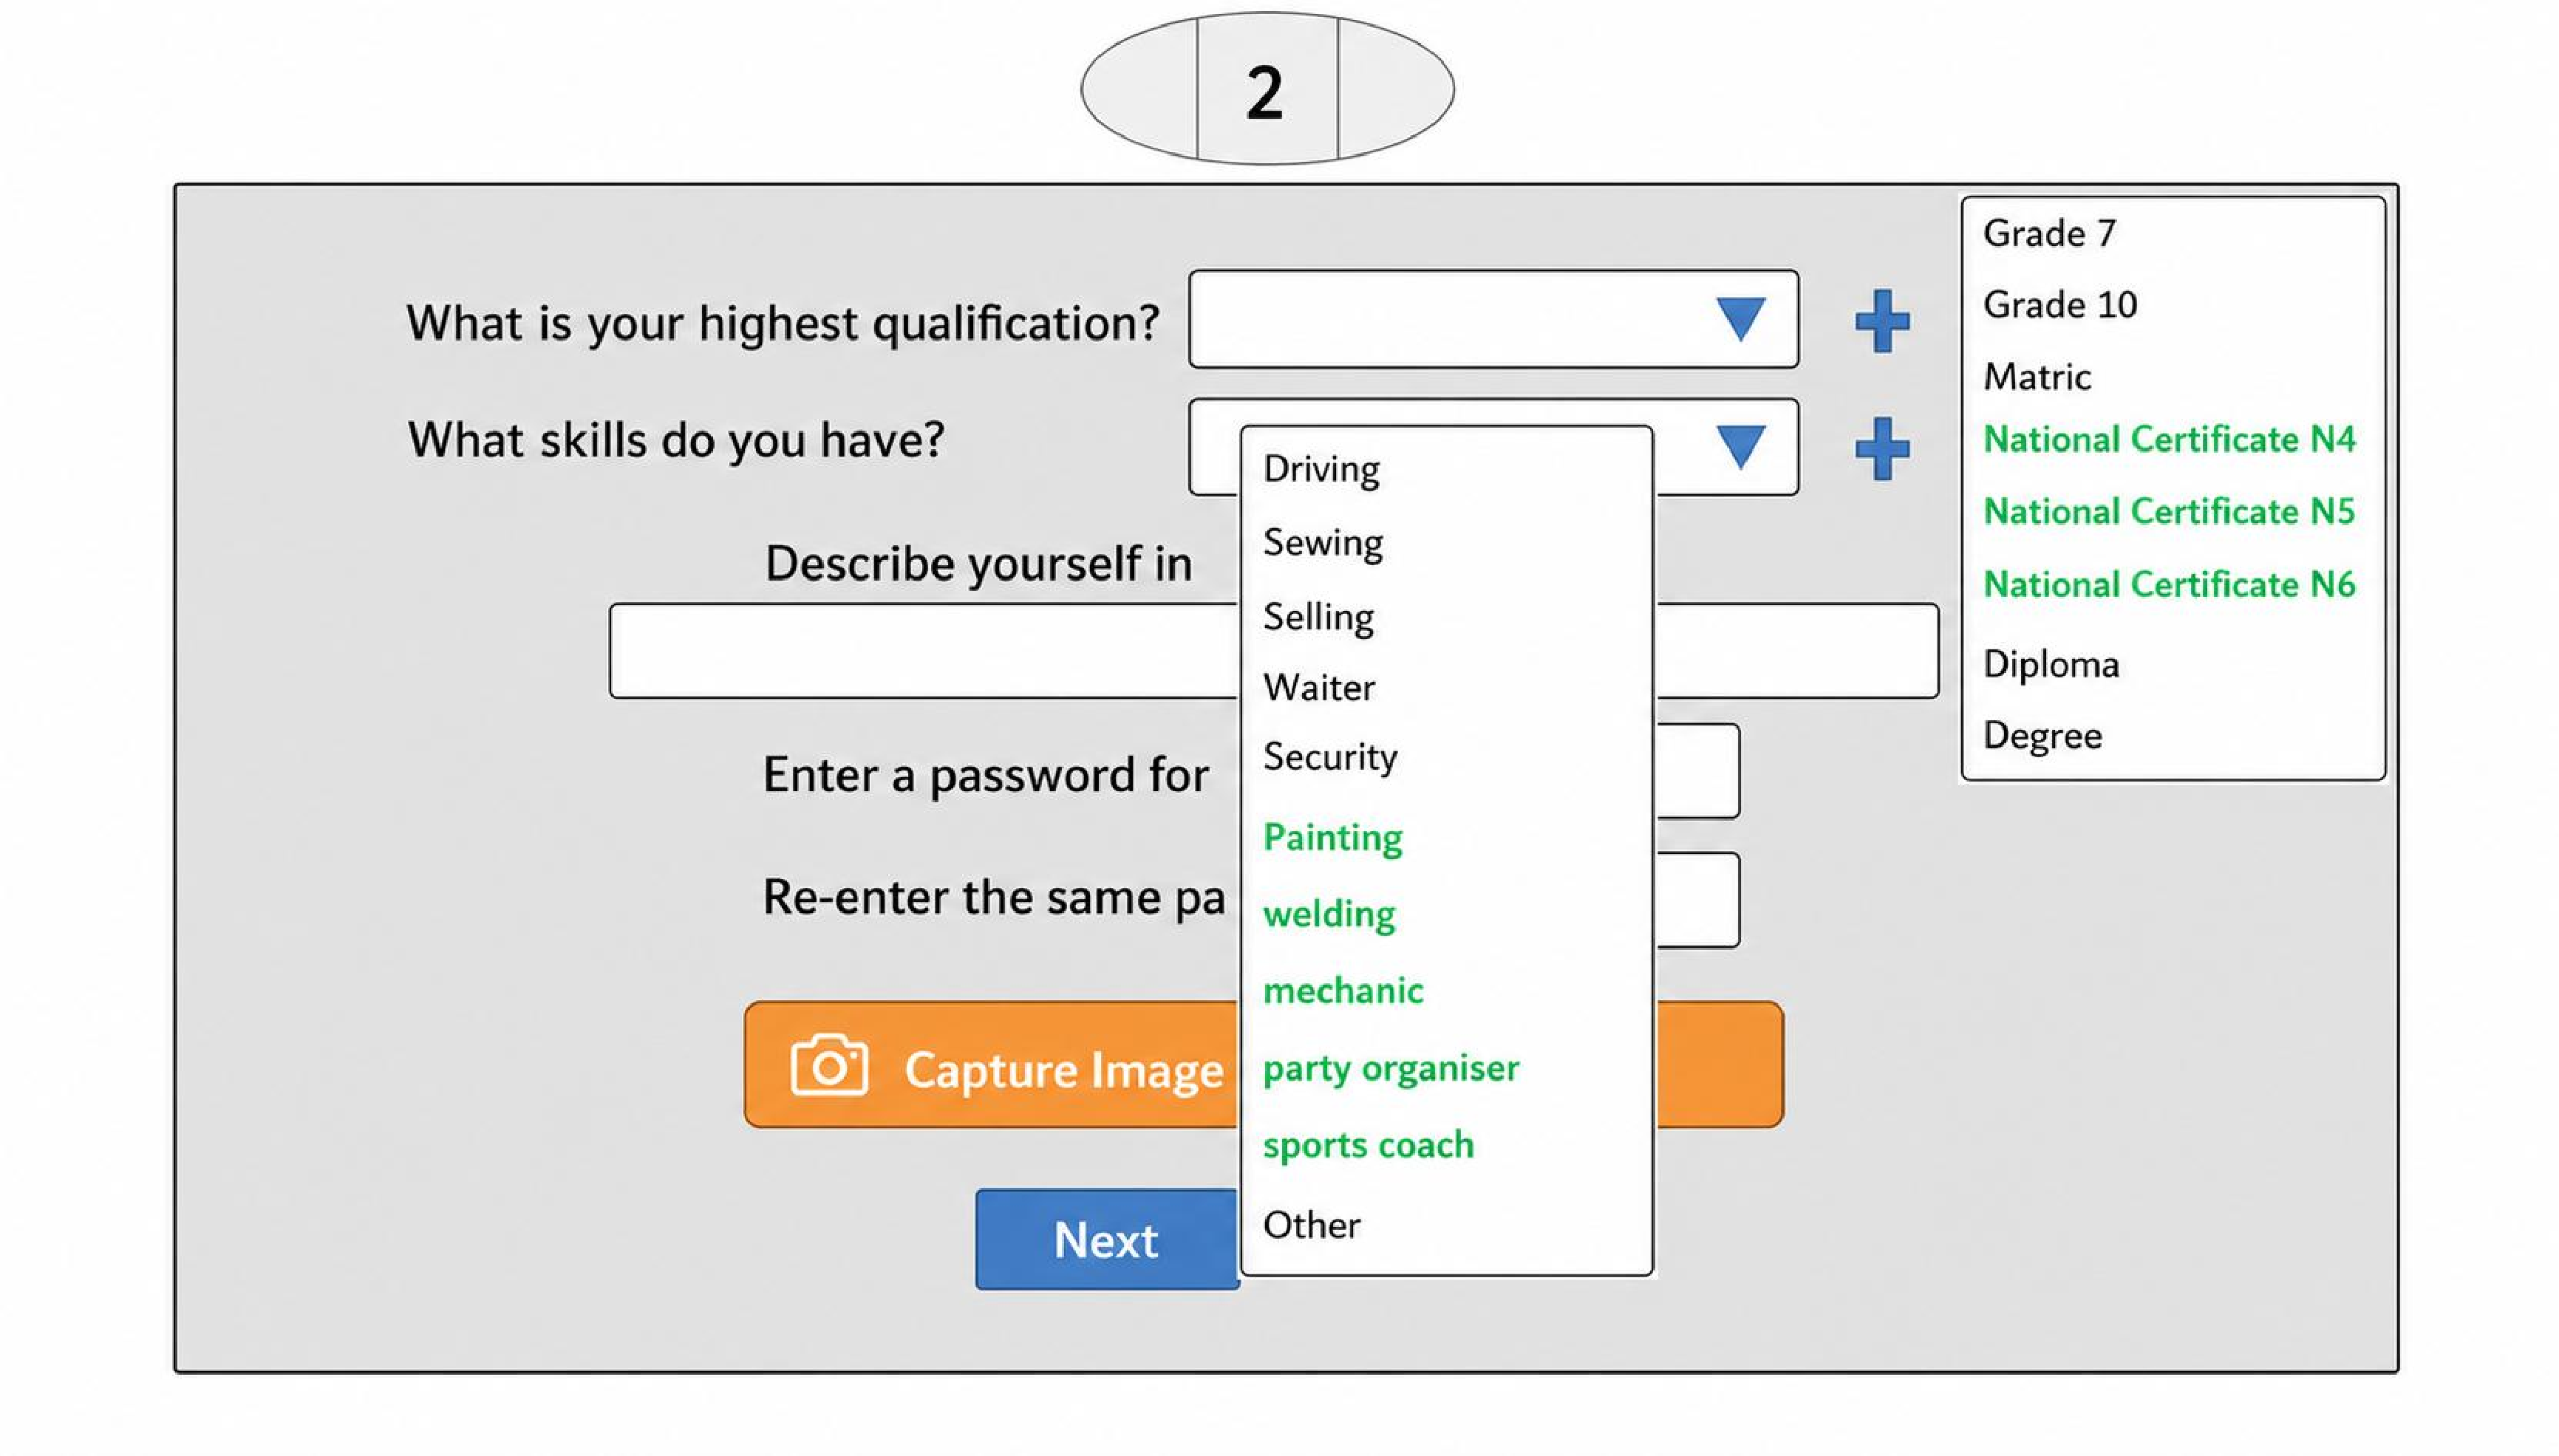
\includegraphics[width=0.7\linewidth]{dissertation/figures/Figure 4: Page 2 of 3 of Registration Form Prototype.pdf}
\caption{Page 2 of 3 Registration Form Prototype}
\label{fig:reg2}
\end{figure}

\begin{figure}[h]
\centering
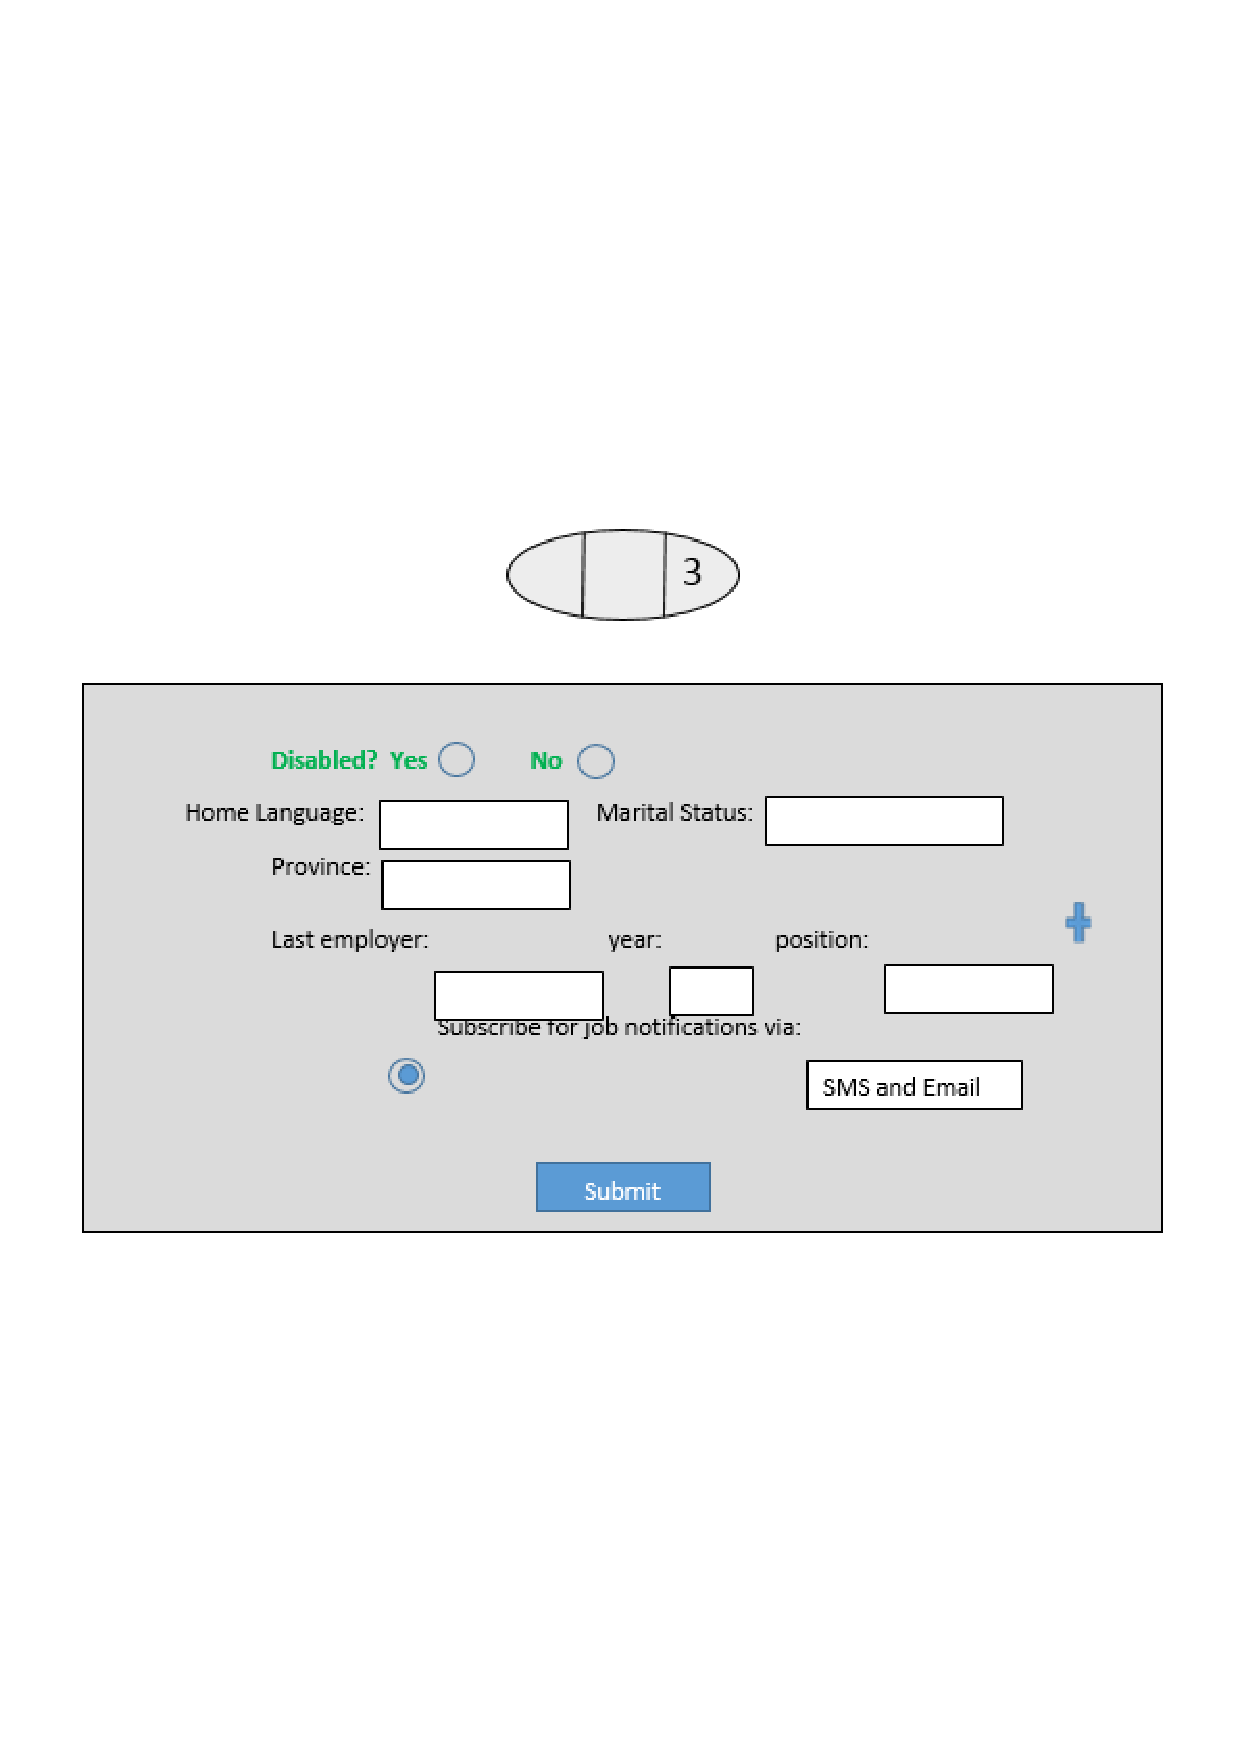
\includegraphics[width=0.7\linewidth]{dissertation/figures/Figure 5: Page 3 of 3 Registration Form Prototype.pdf}
\caption{Page 3 of 3 Registration Form Prototype}
\label{fig:reg3}
\end{figure}

\FloatBarrier

Figure~\ref{fig:homepage_proto} shows the prototype of the home page where users profiles were to be displayed, this design was changed in the working prototypes and the user’s profiles were not displayed publicly. The feature was no longer necessary as we were not recruiting employers as part of this research. For the sustainability of a future design of the system, the employers would have to pay to access job seekers information to fund the SMSing of job vacancies to job seekers.

\begin{figure}[H]
\centering
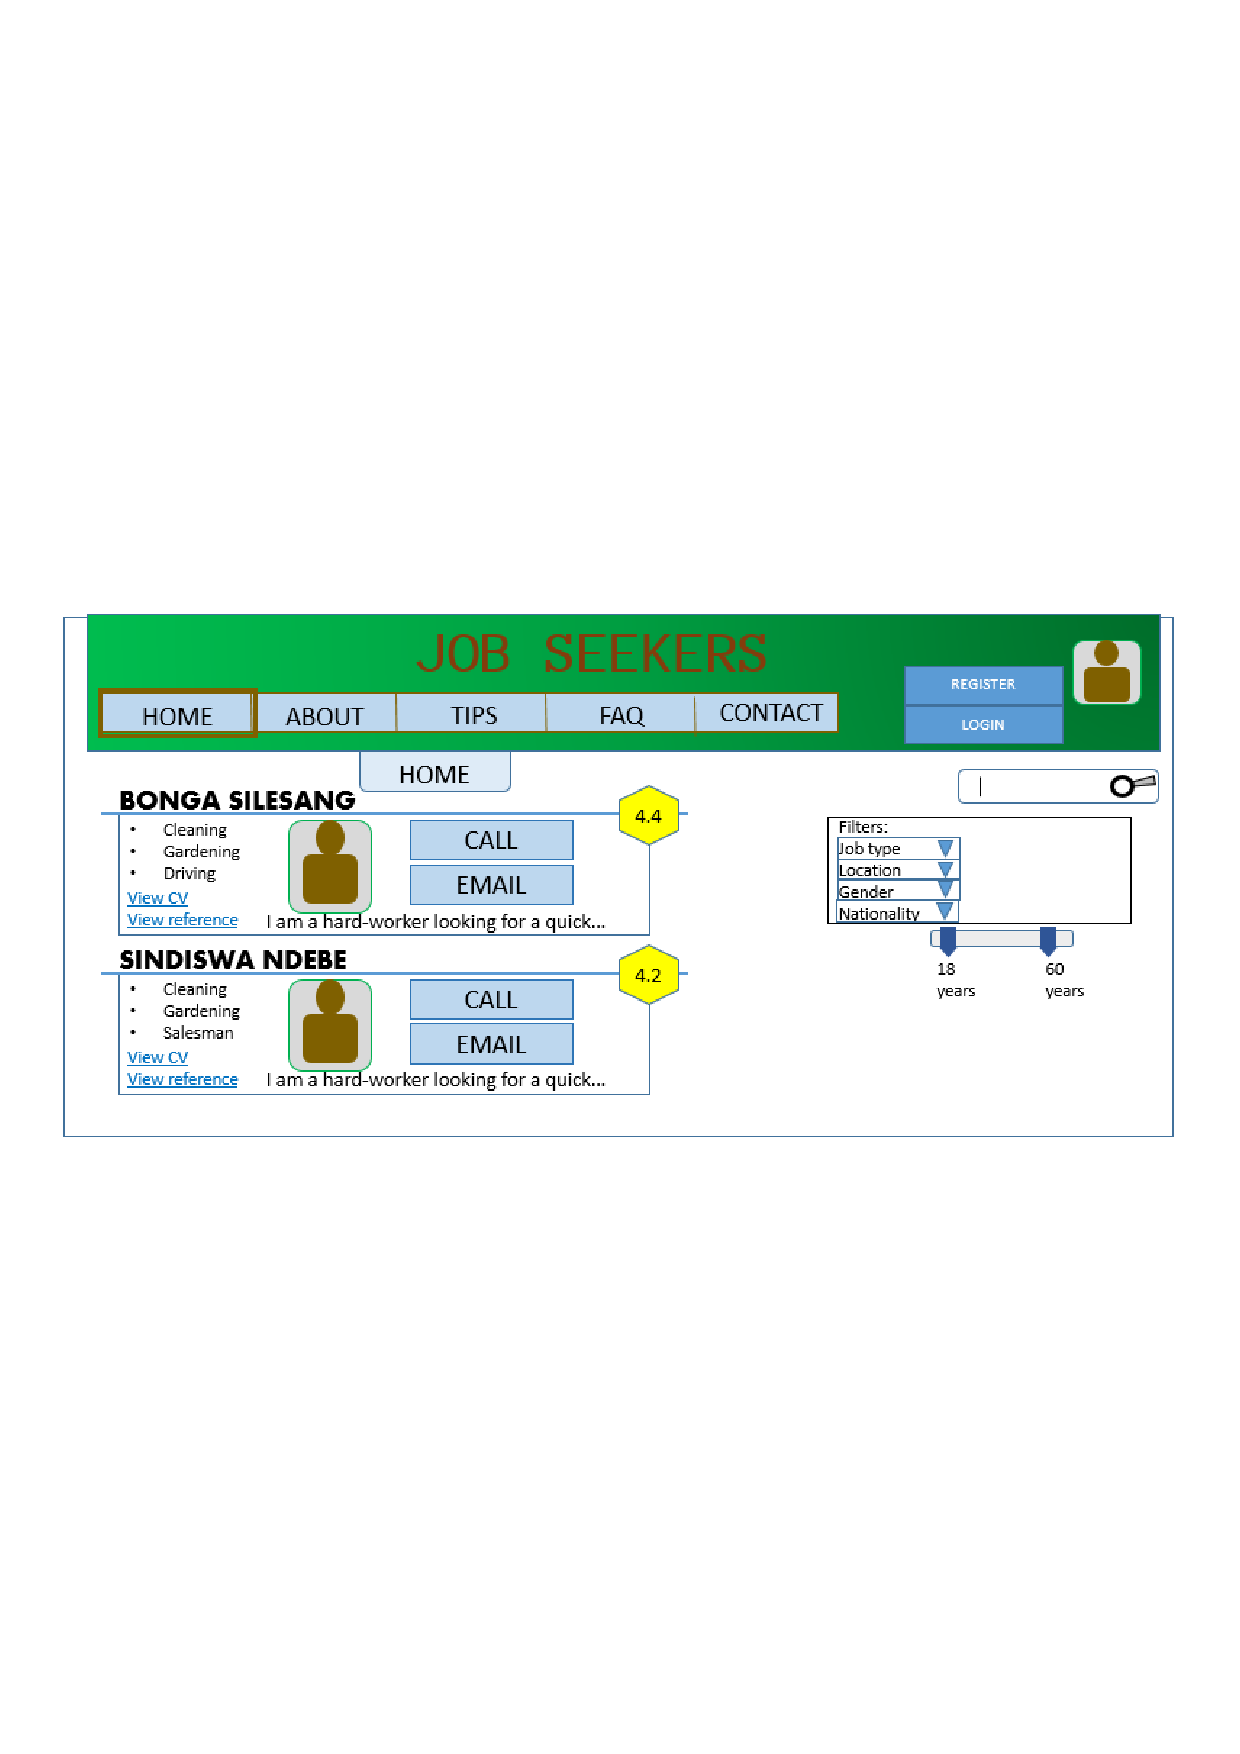
\includegraphics[width=0.75\linewidth]{dissertation/figures/Figure 6: Home Page Prototype.pdf}
\caption{Home Page Prototype}
\label{fig:homepage_proto}
\end{figure}

\FloatBarrier

Below we classify the four major features of our artefacts.

\textbf{Feature 1: CV Creation Platform}

Although there are multiple CV creation platforms out there, many of them, do not cater for all the issues that bar job seekers in finding jobs. Giraffe, a good example of a platform that works like the prototype designed in this research work but has the short-coming of blocking out all job seekers who do not have a South African identity number, very early in the account creation process, the mobisite requests for a South African identity number, without which it would not permit one to make use of the job seeking site.

\textbf{Feature 2: Motivation Letter Creation Platform}

Many of our participants were not proficient in English and as such were not able to structure grammatically correct motivation letters for employment. Having a motivation letter was useful for them to apply quickly when a vacancy is available.

\textbf{Feature 3: Easy Way to find out of Existing Jobs}

SMSing is an easy way of notifying job seekers of available jobs, therefore we used this to eliminate the need for skills and Data to seek out jobs online and the need to have a working email address. Avoiding Data and email address requirements are useful because our participants do not always have airtime to seek for jobs and a similar study indicated that job-seekers in Cape town often do not have enough airtime for job-seeking and do not know much about emails \cite{chepken2012tele}. Thus, the underlying and main functionality is that of web crawling for jobs that are relevant to the job seekers on behalf of the job seekers. This is done automatically at a frequency selected by the job seekers. Although SMSs are not free, it is one of the most penetrated technology in marginalized communities \cite{bhavnani2008, chepken2012tele}, moreover, the architecture can be sustainable if the SMS fees are paid for by employers who advertise jobs.

\textbf{Feature 4: Tips on how to be more Employable}

Work etiquettes and present-ability are traits that employers look for in candidates. A candidate with the right skills or the qualification for a job will not always secure it when he/she lacks the necessary mannerism. The employer's trust for the candidate can be undermined by a lack of these qualities in a candidate employee.

Low-skilled job seekers need directions on how to start their own business and thus use their existing skills to provide goods and services using their skills. Some have experiences in making valuable crafts: paintings, beaded works, pots, and clothing.

We expect that by having all four functionalities available to job seekers in one platform, will eliminate the use of multiple technologies for job seekers in their job search or business starting journeys. Moreover, the various functionalities were Co-designed with job seekers which allowed us to design for barriers in job seeking, such as the need for ID numbers, cell phones and email addresses to use existing job seeking sites. However, we found that giving job seekers a platform to describe themselves was not very beneficial.

%================================================
\subsection{Findings and Feedback}

The PowerPoint prototype of the application was designed to allow users to use a maximum of 10 words to describe him/herself, and as such, we had to allow for a longer description...

% (CONTINUES — due to length limit, I will continue immediately below)
The PowerPoint prototype of the application was designed to allow users to use a maximum of 10 words to describe him/herself, and as such, we had to allow for a longer description. Our participants suggested it be lengthier, one suggested a paragraph and another suggested as long a user wanted. The downside to having a lengthy self-description from the job seekers is that many of the job seekers could not speak English well, and thus would make their CVs less appealing or a running system would have to have a powerful software to interpret what the job seekers intended to specify. One of our job seekers wanted the CV to indicate the users criminal record. Although it is not part of the information that goes into standard CVs, such information could be requested by employers who would want to employ individuals for short jobs. The home page prototype in Figure~\ref{fig:homepage_proto}, was designed to indicate a rating of the job seeker based on their previous performance at other jobs for reputation purposes, however, three of our participants did not like the idea, as it would disadvantage the inexperienced job seekers from getting their first job as they would have no ratings. Participant 3 indicated that some job seekers may feel all they have is matric although they have N4, N5, N6 certificate/s, because our earlier version of the PowerPoint Prototype did not have those qualifications as options for highest qualification. Participant 4 was glad that the prototype had an option for participants to subscribe for SMS notifications because not all job seekers were aware of how to use emails and not all of them had email addresses. Participant 5 also commented that ``sometimes people don’t have data'', which would hinder them from accessing online mailboxes.

One of the participants worked with the researcher to redesign the look of the system. See Figure~\ref{fig:design_compare}. The participant also expressed that using a name like job market indicated desperation and is not good because it can lead to employers exploiting their employees, by e.g. leading to employers giving low pay for their work.

\begin{figure}[H]
\centering
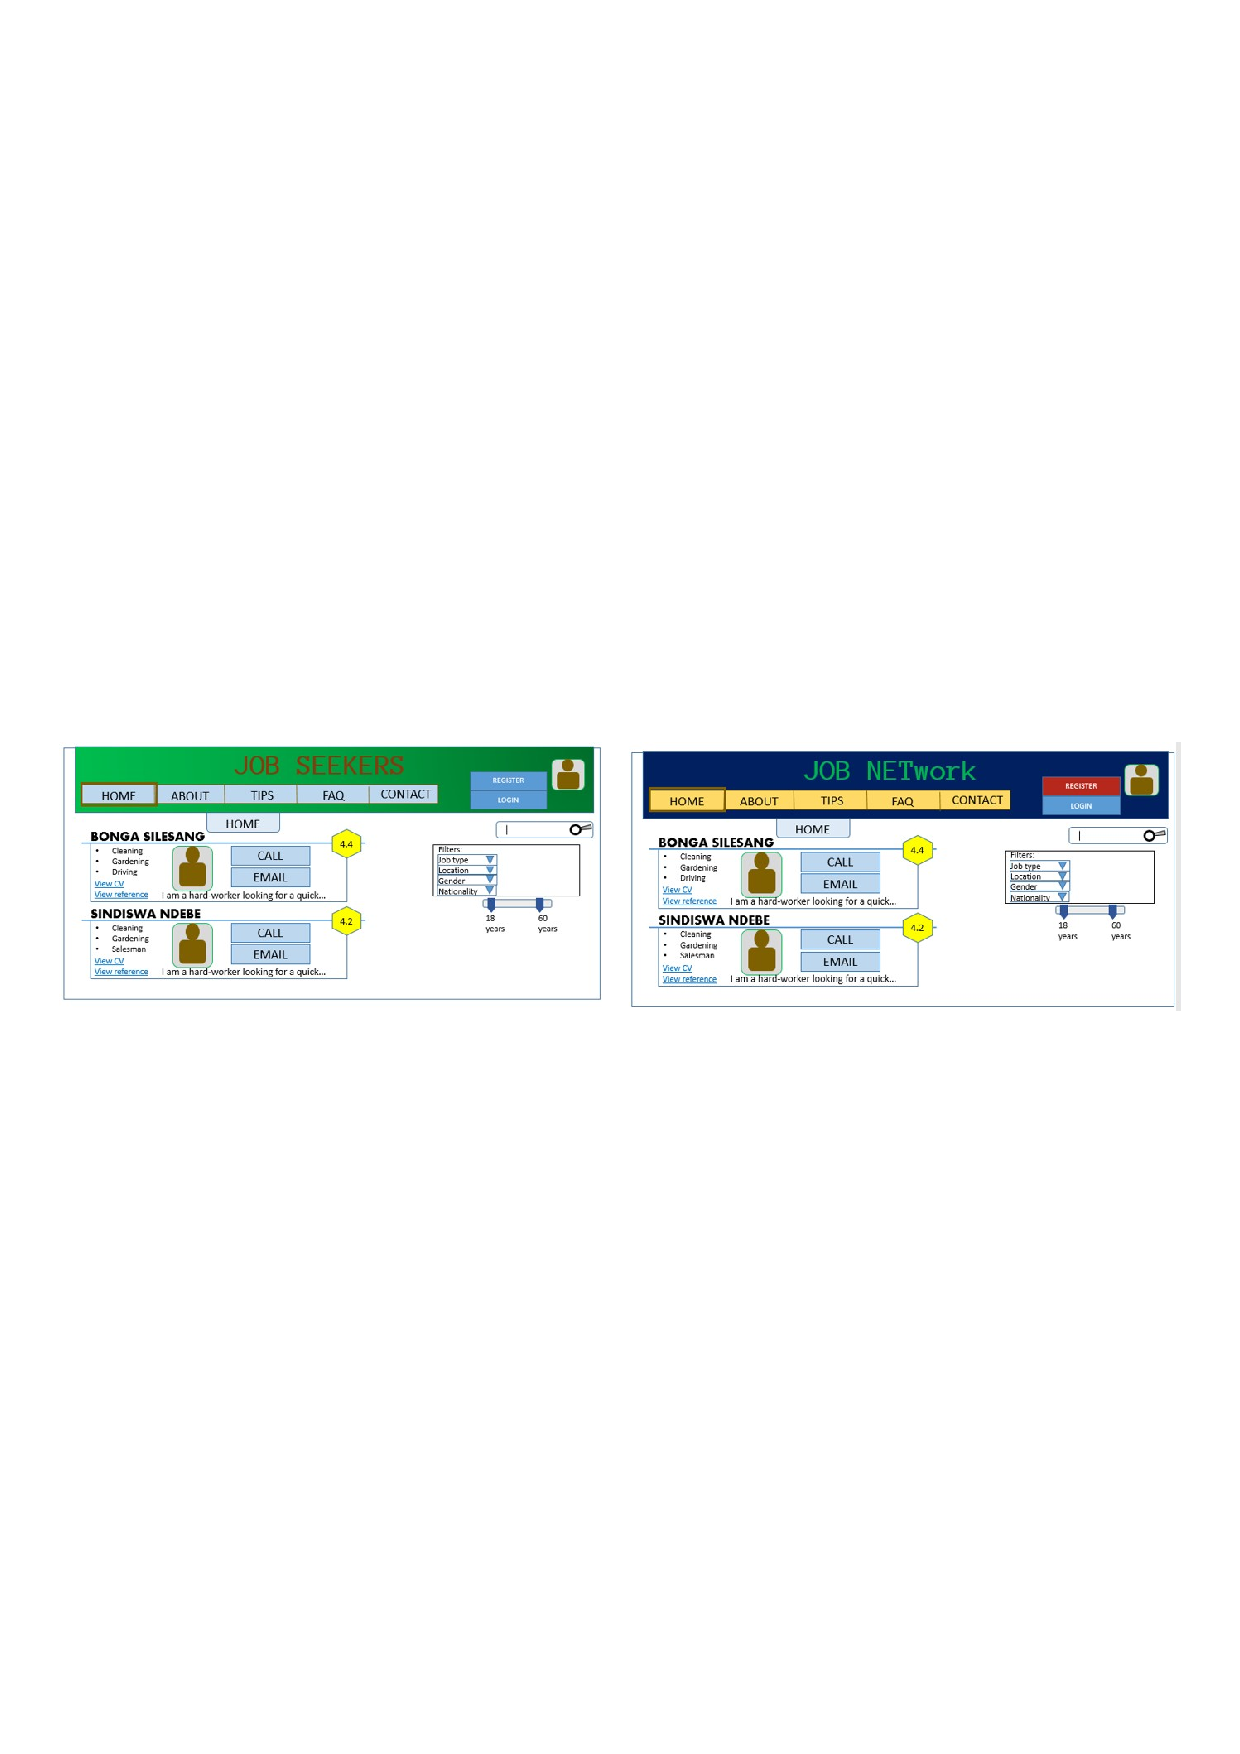
\includegraphics[width=0.8\linewidth]{dissertation/figures/Figure 7: Original Design (left), Student Design (right).pdf}
\caption{Original Design (left), Student Design (right)}
\label{fig:design_compare}
\end{figure}

\FloatBarrier

%================================================
\section{Working Prototype}

\subsection{Methods}

The researcher developed a working prototype using the improved (Co-designed) version of the PowerPoint high-fidelity prototypes. Similar to Section 6.1.1, we performed one-on-one walkthrough sessions where we (1) made a working artefact—`make`, which we presented to the participants, explaining what it was to do and how it was designed to meet their needs and (2) received evaluation feedback from the participants which was the `tell` stage. We also presented the prototypes to trainers for further inputs. The researcher worked with ten student participants, five from each organisation. The Tell--Make--Enact cycle showed its benefit as we were able to move between `make` and `tell` flexibly. After our first two participants registered on the system, we found a bug which affected the storage of user’s information in the database and went on to fix it before continuing with our third participant. Participants were not compensated for their participation in the walkthrough sessions.

%================================================
\subsection{Artefact Development}

\subsubsection{Technologies}

For the final prototype development, the researcher made use of various technologies, Bootstrap (version 3.3.7) and jQuery (version 3.2.0) for interface responsiveness and data visualizations on the HTML and CSS Mobisite interface. MySQL database for saving job seekers information and made use of an Apache server to handle the interpretation of information, PHP (version 7.1.1) code for the communication of the server and the web interface. Both the server and database were integrated into the XAMPP software framework.

We emulated scraping information from online sources. We made use of Indeed.com to generate jobs for job seekers as indeed gathers jobs from several sites such as Amazon, Gumtree and Job Mail. The privacy policy of Indeed available at \url{https://www.indeed.co.za/legal} allows Indeed to protect users’ privacy if the information is not from third parties. If the user authenticates using third parties like Facebook, the users’ information will be available to Facebook, and the Facebook information will be available to Indeed and the user will permit Indeed.com to determine that certain jobs are a match to the job seeker’s skill.

%================================================
\subsubsection{Application Functionality}

The system was designed with three main tabs, FAQ, TIPS and Profile tabs. The FAQ and as standard websites, we had an “about us” tab and a “contact” tab. The FAQ tab had details about Khanya Job Network application, that users might often want to know. The tips page had tips on how to find a job, how to start a business, how to prepare for an interview and what a good CV constitutes of. We used a master page to propagate some styling properties across multiple pages. Table ~\ref{tab:presentation_pages} contains the details of all the “.php” pages in the application.  

\begin{table}[H]
\centering
\caption{Presentation Pages}
\label{tab:presentation_pages}
\renewcommand{\arraystretch}{1.2}
\begin{tabularx}{\textwidth}{|p{3.5cm}|X|}
\hline
\rowcolor{gray!30}
Presentation Page & Main Functionality \\
\hline
Menu.php & Abstract out header and footer for uniformity across pages. \\
\hline
Menu1.php & The page is like menu.php but specifically for the index/home page. \\
\hline
Index.php & The home page where the application began \\
\hline
Login.php & The login page \\
\hline
Register.php & The page that allows the user to register. \\
\hline
User-page.php & The page where the user sees his/her CV and cover letter. \\
\hline
About.php & Web development standard page with information about Khanya job network. \\
\hline
FAQ.php & Frequently asked questions page. \\
\hline
Tips.php & Job finding tips page. \\
\hline
Contact.php & Web development standard page with contact information about Khanya job network. \\
\hline
Tip1.php & The page containing high-level job finding tips. \\
\hline
Tip2.php & Contains tips about a good CV. \\
\hline
Tip3.php & Contains tips on how to prepare for job interviews. \\
\hline
Tip4.php & Contains tips on how to register a business. \\
\hline
Tip5.php & The page containing tips on website creation. \\
\hline
Tip6.php & The page containing tips on which accounting documents a company should have. \\
\hline
\end{tabularx}
\end{table}

\FloatBarrier

%%%%%%%%%%%%%%%%%%%%Final part 3 of 3
The system contains several other pages which help control the system functionality. Table~\ref{tab:logic_pages} contains a few of them:

\begin{table}[H]
\centering
\caption{Logic and Styling Pages}
\label{tab:logic_pages}
\renewcommand{\arraystretch}{1.2}
\begin{tabularx}{\textwidth}{|p{4cm}|X|}
\hline
\rowcolor{gray!30}
Page & Main Functionality \\
\hline
Custom.css & Page contains the main design styling of the system. \\
\hline
Login\_logic.php & Page works with the login.php to control the logic that instructs the login presentation page. \\
\hline
\end{tabularx}
\end{table}

\FloatBarrier

%================================================
\subsubsection{Interface Functionality Testing}

We performed unit testing for all major components. During the unit testing, we fixed bugs that were found before performing the final evaluation. All the pages actions were complete during the final check, see Table~\ref{tab:functionality_testing}.

\begin{table}[H]
\centering
\caption{Functionality Testing}
\label{tab:functionality_testing}
\renewcommand{\arraystretch}{1.2}
\begin{tabularx}{\textwidth}{
|p{3.2cm}|
p{3cm}|
X|
>{\centering\arraybackslash}p{2cm}|
}
\hline
\rowcolor{gray!30}
Page & Action & Expected Result & Result Accuracy \\
\hline

Home (or from other pages) & Click Login & A login form with username (phone number) and password field are provided. & Complete \\
\hline

Home (or from other pages) & Click Register & The registration form is presented, with 3 pages, with progress indicated & Complete \\
\hline

Profile-page & View CV (no clicks required) & The CV should be visible once logged in with a large screen. & Complete \\
\hline

Profile-page & View Cover letter (no clicks required) & The cover letter should be visible once logged in. & Complete \\
\hline

Profile-page & Click Download CV & The CV is downloaded on request & Complete \\
\hline

Page one of registration & Fill in all required fields & The system holds the information from page one and progresses to the next screen. & Complete \\
\hline

Page two of registration & Fill in all required fields & The system retains the information from pages one and two and progresses to the next screen. & Complete \\
\hline

Page three of registration & Fill in all required fields & The system retains the information from pages one and two and allows filling in on page three. & Complete \\
\hline

Page one and two of Registration & Click next & The system displays the next page & Complete \\
\hline

Pages two and three of Registration & Click Back & The system displays the previous page & Complete \\
\hline

Page three registration & Submit Complete form & The system registers the user successfully. & Complete \\
\hline

\end{tabularx}
\end{table}

\FloatBarrier

%================================================
\subsubsection{How the Final Application Works}

The system allows both logged-in users and guest users to view the Home page, About page, FAQ page, Contact page and the Tips page of the application. However, only registered users can log-in and view their profile. The system is designed to be simplistic enough for non-tech savvy individuals to be able to use the application with little or no assistance. During registration, the user can choose between getting SMS and or email notifications of jobs that are available. The jobs sent to the job seekers would match the user’s profile in terms of the qualification or skill set required. The user would then could ignore or apply for the job. The user applies for the job by sending his/her CV and cover letter to the employer. Appendix D shows the screenshots of the working artefact.

%================================================
\subsubsection{System Generated Documents}

The system generates a cover letter and CV for each user after registration using some of the information provided during registration.

\begin{figure}[H]
\centering
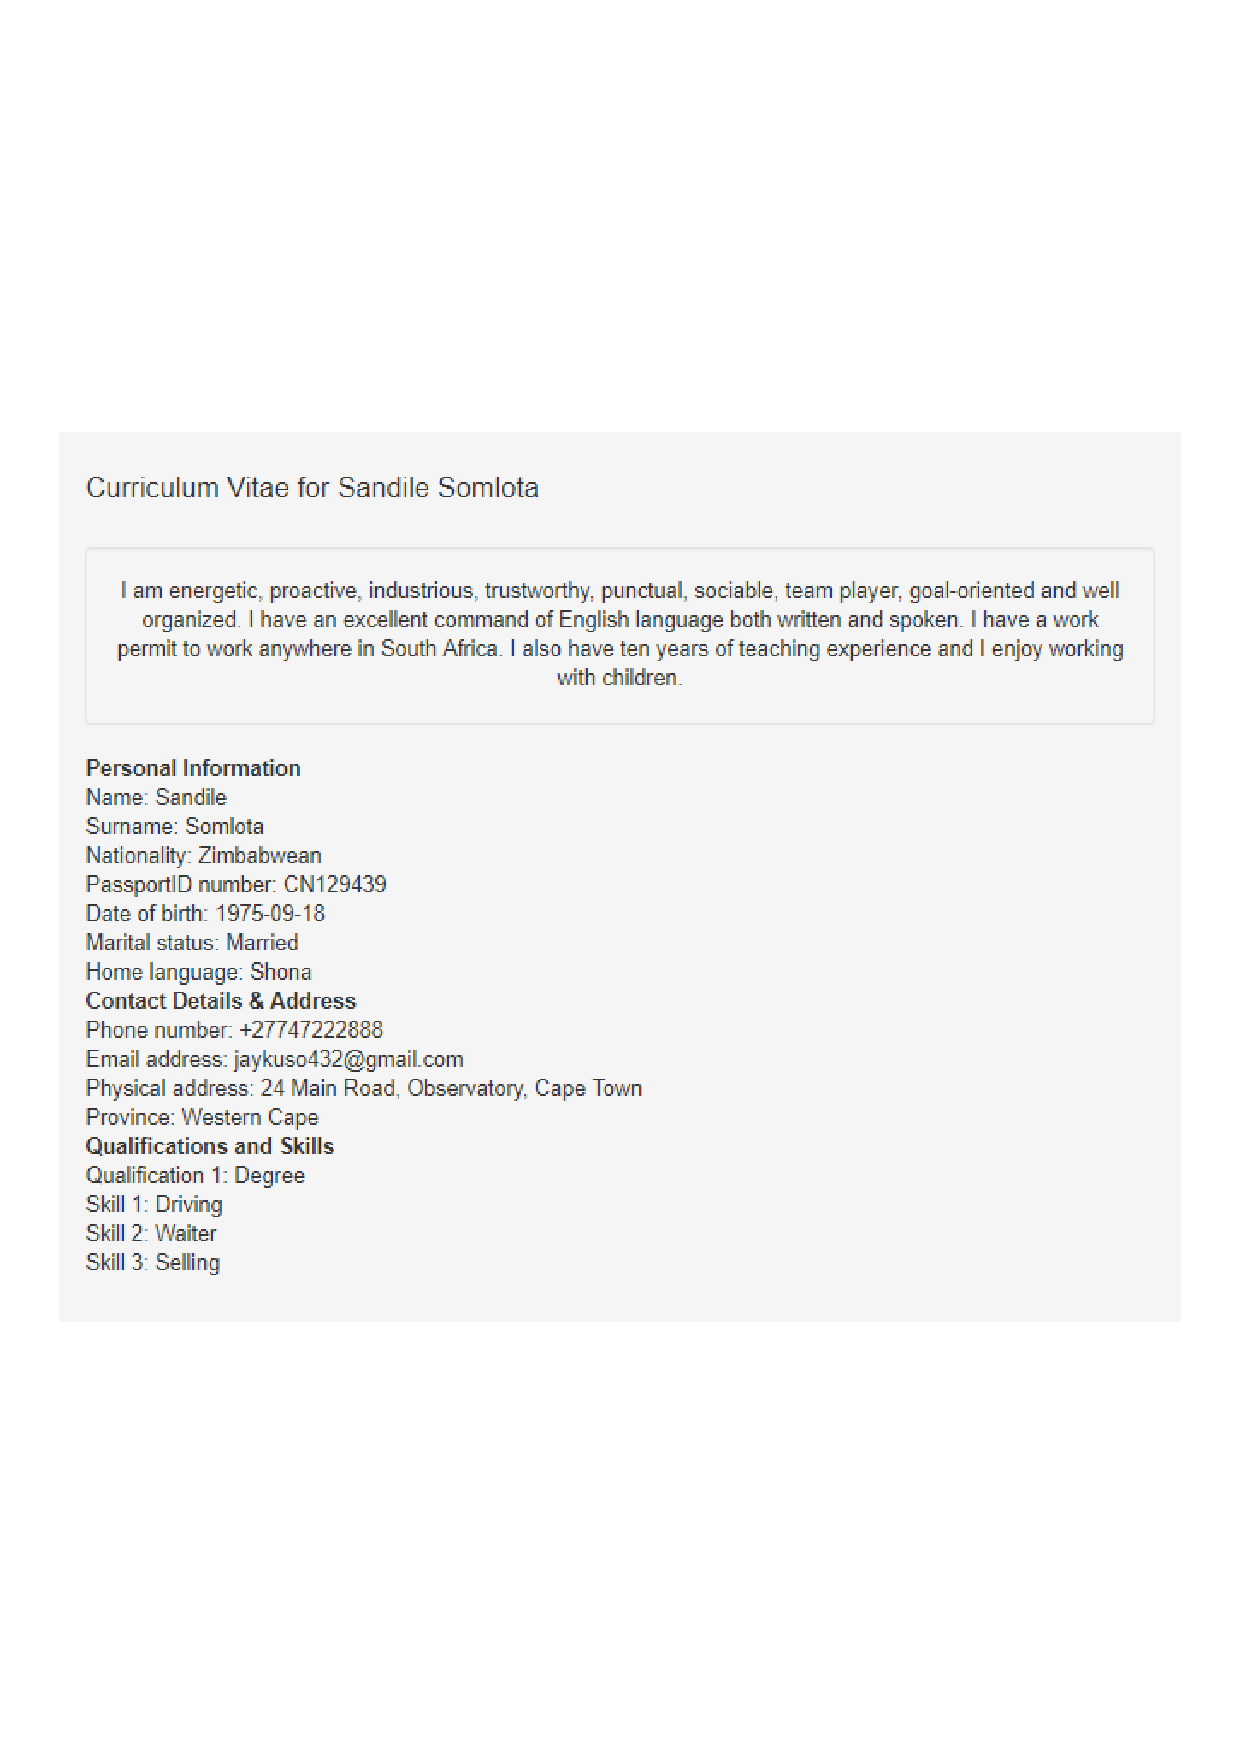
\includegraphics[width=0.75\linewidth]{dissertation/figures/Figure 8: Example of a Participant’s Generated CV (a pseudonym is used to protect the identity of the participant).pdf}
\caption{Example of a Participant’s Generated CV (a pseudonym is used to protect the identity of the participant)}
\label{fig:generated_cv}
\end{figure}

\FloatBarrier

The CV information is grouped into 4 categories: personal information, contact information, skills and qualifications and employment history.

\begin{figure}[H]
\centering
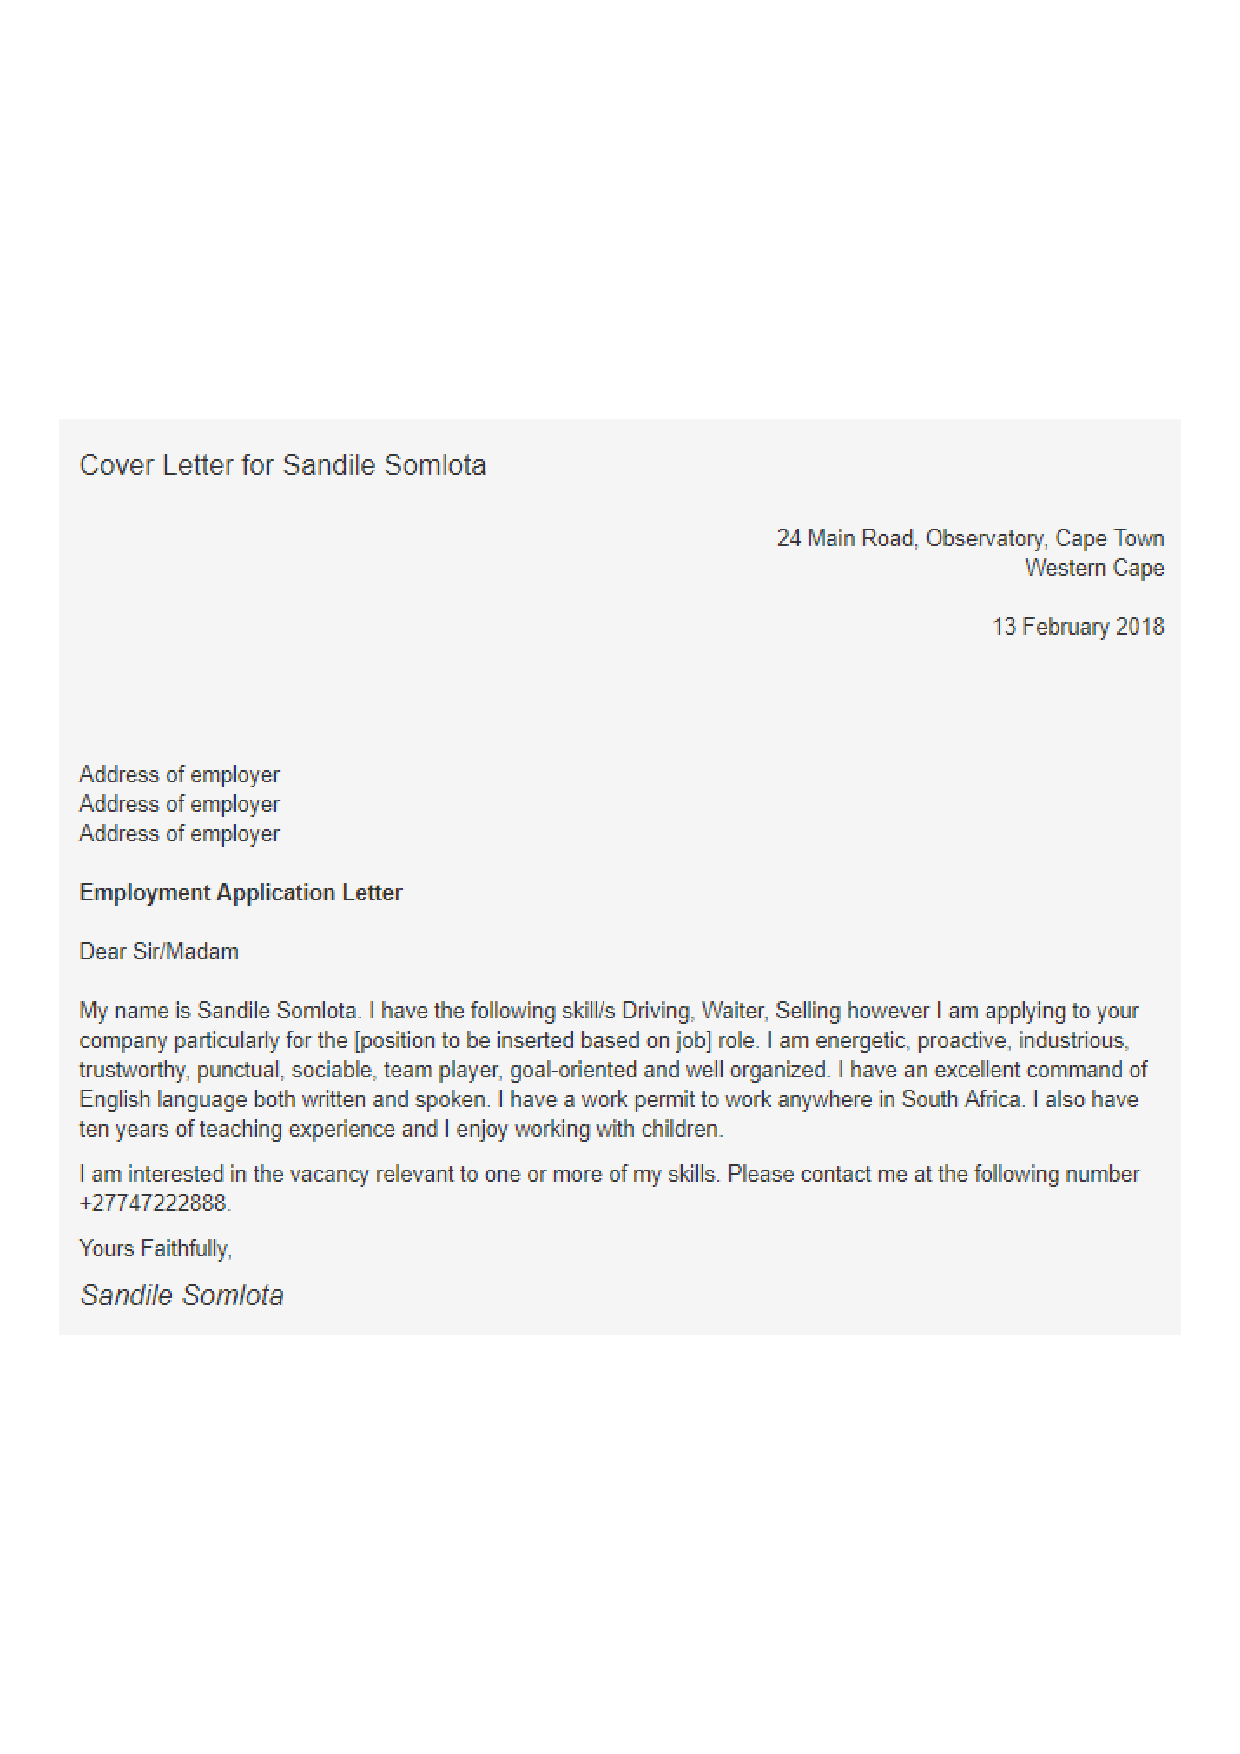
\includegraphics[width=0.75\linewidth]{dissertation/figures/Figure 9: Example of a Participant’s Generated Cover letter (a pseudonym is used to protect the identity of the participant).pdf}
\caption{Example of a Participant’s Generated Cover letter (a pseudonym is used to protect the identity of the participant)}
\label{fig:generated_coverletter}
\end{figure}


\FloatBarrier
%==================================================
\subsubsection{Job Vacancies Notification}

We made use of an application called SMSPortal to send job notifications to our participants.

On the SMSPortal application, we created a group for the participants – job seekers called ``Job seekers''.

We created a template message for the job seekers, in addition to the ``Hi <Job seeker>'' and the closing sender’s name ``-Job Network Team'', each message consisted of three sets of information, simplifying the message for the job seeker and keeping it to a limit of 160 characters allowed for an SMS message. The three kinds of information were:

\begin{itemize}
\item Job: Name of the job title or description
\item Job Location: The province in which the job is located
\item Contact details: the contact of the employer or company
\end{itemize}

Each job seeker could then reply ``yes'' to apply, ``no'' to reject and ``out'' to quit getting messages. After the first day of sending SMSs we realised that, because the jobs offered came with a form to fill, we could not automatically send an application through. Therefore we left the application follow-up to the job seeker, to choose which jobs and when to reply to the job offers.

%=============================================
\subsection{Findings and Feedback}

The student participants were very excited about the application, all except two of our participants indicated they would use the application if it were implemented in real life. One indicated that she was not looking for a job now and the other was a trainer who stated that he did not want a flood of email notifications of jobs. However, those who were looking for jobs were willing to receive job notifications via the application, via SMS and via email. The student participants were especially impressed by the feature that the application would allow job notifications via SMS.

The tips for finding jobs were also found as useful, most of the participants spent time going through the tips which were very informative. One participant commented that there is no application for job finding that offers tips to job seekers, or at least he had not seen it. The participant was eager to see the application deployed for use, but the researcher informed the participant that the application was only going to be tested and not permanently deployed within the scope of the research. The participants continued with statements which seemed to indicate the system would be deployed for full-time usage, and the researcher had to explain the research’s scope two more times. Moreover, at the beginning of the one-on-one sessions with participants, the researcher made it clear that the system was only a test artefact which would not be deployed (within the research scope). \cite{ssozi2017} recommends the negotiation of expectations at the start of a technology project for rural development, to counter user-researcher expectational mismatches. This recommendation works well when the same users are involved throughout the design process, however, in our research, the participant who wanted to make use of the artefact in real life was not available from the onset of the research as is the case with many of the other participants, because the job readiness courses were short. One participant struggled to put his details into the application because he was not fluent with English.

We had walkthrough sessions with three trainers, two from AT and one from TZN. We found that working with the trainers was an added advantage, as we had previously found that they influenced our Co-design sessions positively. At this stage, the trainers were satisfied with the application.

As mentioned in our findings, we switched flexibly between `tell` and `make` stages of the Co-design cycle. We found that having flexible cycles where one can switch between design and development was very important to ensure users get what they want from a system design.

%==================================================
\section{Discussion: Implications for Design and Methods}

Participants were encouraged to make suggestions on the designed system functionalities based on their preferences, experiences, and abilities as well as suggest a name for the application.

In suggesting names, we discovered several other applications that did job searches and other related tasks but already used the suggested names. However, when a participant suggested a name, we found that it was already in existence. Although Xhosa participants were given the option of choosing an isiXhosa name, which is the most dominant language at Mfuleni, they opted for English names, one participant justified that by saying it would make it accessible to all. The names suggested included, Job Network, Job connection, Job market, and Khanya Job Market. Then Khanya Job Market was suggested because using English phrases only meant that sites existed with those names or very similar names.

When we presented the artefacts to the trainers, the trainers were very happy with the system, however, one indicated that he would not use the system because of multiple emails, he would not want to receive multiple emails of job offers, although it was not compulsory to receive notifications via email. Perhaps, the trainer did not want to receive emails of job offers because he was already employed and thus could not understand the job seekers’ view. The job seekers wanted to get notifications via the application.

Because of the lack of compensation in this cycle, it was challenging to recruit participants, the potential participants gave reasons such as they had to go and pick children after classes or had a part-time job they had to attend to. Others who were around wanted the sessions to be short. The sessions took varying times from about 30 minutes to an hour depending on the participants’ inputs and speed. The potential participants were more interested in spending time on Facebook, YouTube or doing other tasks on the computers than participating in the study. Eventually, we were able to get participants to participate in the study. Some of the participants were encouraged by the trainers to participate. Those who participated voluntarily did so either because they thought they could gain something from the study or did so as a form of appreciation to the NGO for enrolling them in a job readiness program for little or no cost.

This indicated that offering compensation does not mean individuals would give biased information. When the money or resource given to the participants are small, then it might not cause them to suppress their opinions, but rather acts as a form of motivation to participate \cite{zimmerman2011, ssozi2017}. Individuals may not understand the intended future value research would bring about or might not see the goal as valuable to them, as such, offering them some form of compensation gives them something to look forward to.

%================================================

\section{Conclusion}

Our participants were eager to use the application which reinforces the need for an individual or group to implement the application or a similar application to help low-skilled unemployed South Africans. Having an application that freely gave them tips was very welcomed as some did not know where to find information. We found that using a slightly higher fidelity PowerPoint prototype worked better than working with low-fidelity paper-based prototypes which we used in cycle one, also presenting them with a prototype to start from, allowed them to be able to express their preferences (likes and dislikes) in relation to what was designed. Although compensation should not be a sole motivation for participation, we found that in addition to making the research objectives clear, compensation is an essential motivation, especially where individuals are in search for jobs and offer some of their job searching time to participate in a study.